\chapter{Introduction} \label{ch:introduction}
This thesis begins with notations that would be used through out this document.
\section{Notation}
Some standard mathematical notations as well as some non-standard mathematical notations are introduced here.

Angle brackets $\langle \cdots \rangle$ denote a tuple which is to be regarded as a column
vector. The column vector of all 1s is denoted by $\bm{1}$. Transpose is indicated with superscript $T$. 
The standard vector norm is $\|x\| \;=\; \sqrt{x^T x}$. Modulus (or absolute value) is denoted by $|\; \cdot \;|$. 
When $S$ is a set, $|S|$ denotes the cardinality of $S$.

The notation $O(f)$ denotes a function (with similar domain and codomain as
$f$), let's say $g$, such that pointwise $|g| \;\leq \;c |f|$ for some constant $c$. 
Curly brackets $\{\cdots\}$ are used as grouping symbols and to specify both sets
and multisets. Square brackets $[ \cdots ]$ are, besides their standard use as specifying 
a closed interval of real numbers, used to denote an indicator function:
if $expr$ is an expression which may be true or false, then
$[\mbox{\em expr\/} ]$ denote $1$ if {\em expr\/} is
true, and $0$ otherwise. $[ \cdots ]$ is sometimes referred to as an {\em Iverson bracket}. 

The supremum is the least upper bound, and is denoted by sup. The in mum
is the greatest lower bound, and is denoted by inf.

$\mathcal{R}$ is the set of haploids (i.e., length $\ell$ binary strings), and is a
commutative ring $\mathcal{R}$ under component-wise addition and
multiplication modulo $2$. If $x \in \mathcal{R}$, then $x = \langle x_0, x_1, \cdots, x_{\ell - 1} \rangle$. 
Denote the additive identity by ${\bf 0}$ and the
multiplicative identity by ${\bf 1}$, and let $\overline{g}$
abbreviate ${\bf 1} + g$.  Except when explicitly indicated otherwise,
operations acting on elements of $\mathcal{R}$ are as defined in this
paragraph. In particular, $g \overline{g} = {\bf 0} = g+g$,
  $g^2 = g$, $g + \overline{g} = {\bf 1}$ for all $g \in
  \mathcal{R}$.
  
The notation $\theta(x)$ is a function such that $c_0 x \;\leq\; \theta(x) \;\leq\; c_1 x$. 

\section{Background}
The genetic algorithm (GA) is inspired by nature, and seeks to evolve useful constructs. It is population based, and 
proceeds over a number of generations to evolve solutions to problems not yielding to other known methods. 
Basic elements of a GA are: 
populations, selection according to fitness, crossover and random mutation (see \cite{Mitchell1999}). 
Populatoin members are typically fixed length binary strings.   
The fitness function assigns a score (fitness) to the elements (chromosomes) of 
the current population. The simplest form of genetic algorithm involves: selection, crossover, and mutation.

\textit{Selection}: select population members in the current population for reproduction. 
Member with higher fitness are more likely to be selected to reproduce.

\textit{Crossover}: with some probability (the crossover rate), chooses a random (but same point) in two selected members for reproduction 
and exchanges subsequences after that point to create two offspring.

\textit{Mutation}: flip the bits of an individual with some small probability, 
the mutation rate.

Figure \ref{FiniteGA} shows procedural flow of a finite population genetic algorithm.
\begin{figure}[H]
\begin{center}
\resizebox*{10cm}{!}{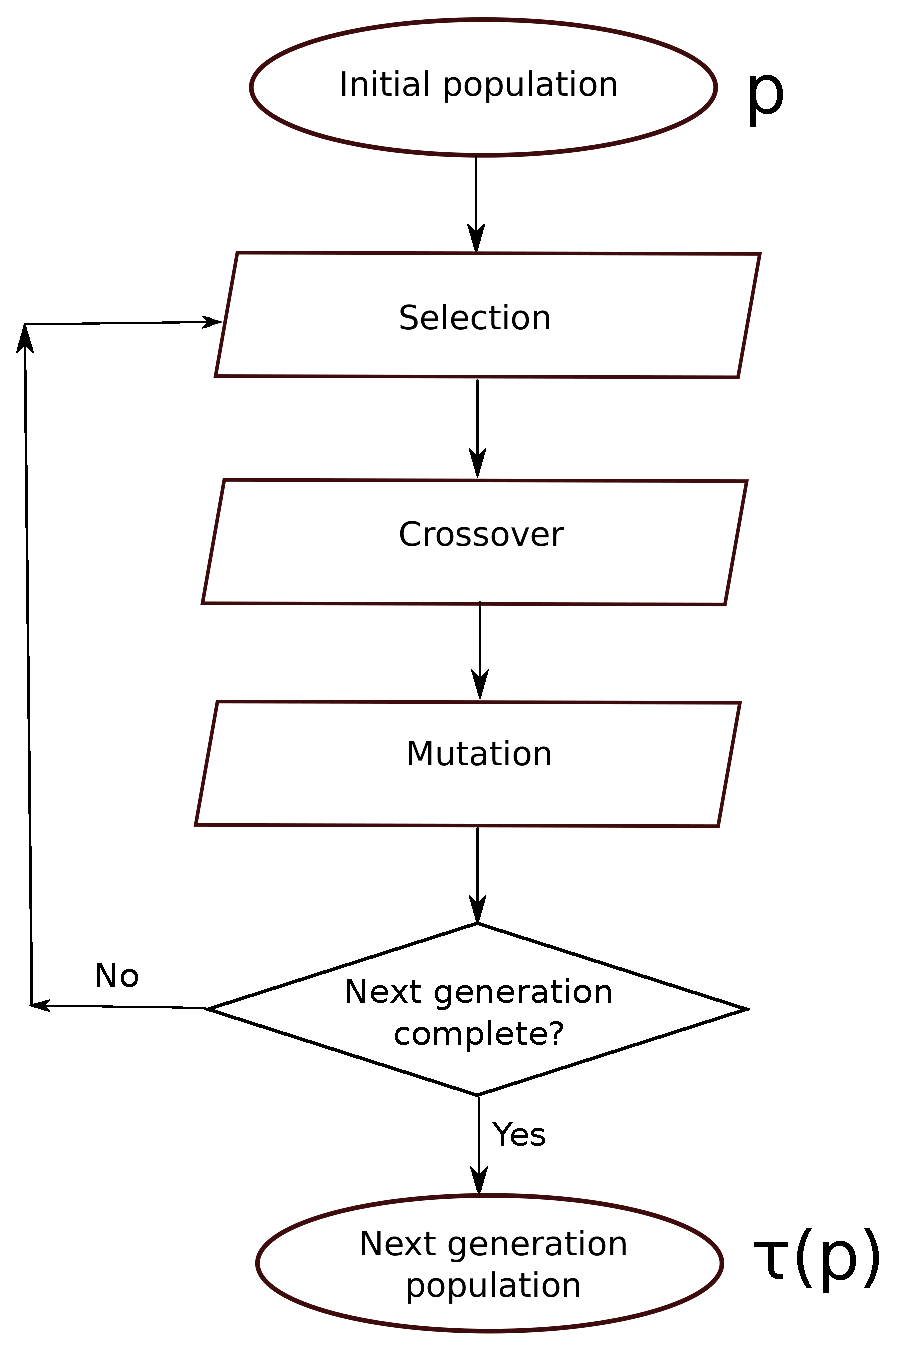
\includegraphics{figures/eps/GA.eps}}\hspace{4pt}
\caption{\textbf{Finite GA} }
\label{FiniteGA}
\end{center}
\end{figure}

A simple Holland style genetic algorithm (see \cite{Holland1975}) works as:
\begin{algorithm}
\label{realGA}
\caption*{A simple genetic algorithm}
\begin{algorithmic}[1]
\Statex 1. Start with some initial population $P$ containing $r$ binary strings of length $\ell$.
\Statex 2. Choose (with replacement) parents $u$ and $v$ from the current population $P$ (using any selection scheme).

  \Statex \hspace{\algorithmicindent} a. Cross $u$ and $v$ to produce children $u^\prime$ and $v^\prime$.
  \Statex \hspace{\algorithmicindent} b. Mutate $u^\prime$ and $v^\prime$ with some probability to produce $u^{\prime\prime}$ and $v^{\prime\prime}$.
  \Statex \hspace{\algorithmicindent} c. Keep, with uniform probability, one of $u^{\prime\prime}$ and $v^{\prime\prime}$ for the next generation
 
\Statex 3. If the next generation contains fewer than $r$ members, repeat step 2.
\Statex 4. Replace $P$ by the new generation formed and go to step 2.
\end{algorithmic}
\end{algorithm}

Each iteration of this process is called a generation. 
The process is repeated until the system stops to improve or some threshold is met.

The infinite population GA models a population as a probability vector $\bm{p}$ where component $\bm{p}_j$ 
is the proportion of string $i$ in the population. If $\mathcal{G}$ is the function mapping current infinite population $\bm{p}$ to 
the next generation, $\mathcal{G}(\bm{p})$ is a probability vector such that 
\[
\mathcal{G}(\bm{p})_j \; = \; \text{the probability that string $j$ occurs in the next generation}.
\]
The evolution of infinite population from an initial population $\bm{p}$ is the sequence
\[ \bm{p} \to \mathcal{G}(\bm{p}) \to  {\mathcal{G}}(\mathcal{G}(\bm{p})) \to... \]

Several people working in the 1950s and the 1960s - like Box (1957), Friedman (1959),
Bledsoe (1961), Bremermann (1962), and Reed, Toombs and Baricelli (1967) developed evolution-inspired algorithms, 
but little attention were given to them (see \cite{Mitchell1999}). Genetic algorithms were popularized by Holland 
and his colleagues in the 1960s and the 1970s. Holland introduced a population-based algorithm with crossover and mutation, 
and promoted his schema theorem ( see \cite{Holland1975}) as providing some perspective on the expected next generation. 
Holland's Schema theorem provides a lower bound for schema survival in 
next generation. A schema is a template that identifies a set of strings in the population with similarities 
at certain string positions; it is made up of $1$s, $0$s, and $\ast$s where 
$\ast$ is the 'don't care' symbol that matches either $0$ or $1$. The schema theorem of Holland is an inequality, 
and does not compute expectation of strings in next generation. 
Bethke (see \cite{Bethke1981}) gave equations for computing the expected number of any string in next generation. 
Goldberg (see \cite{Goldberg1987}) used equations 
for the expected next generation to model the evolutionary trajectory of a two bit GA under crossover 
and proportional selection. Vose and Liepins (see \cite{VoseLiepins1991}) simplified and extended 
these equations by integrating mutation into the recombination of arbitrarily long binary strings. 
Their model computes infinite population trajectories through time. 
Given a finite population with proportional representation vector $\bm{p}^n$ at generation $n$ 
(component $\bm{p}_i^n$ is the proportion of string $i$ in finite population) the infinite population model 
can be used to compute the expected proportion $\bm{p}_i^{n+1}$ of string $i$ as result of \textit{selection} and 
\textit{mixing} in next generation.  
If $\bm{r}_{i,j}(k)$ is probability that parents $i$ and $j$ recombine to produce child $k$, and $\bm{s}_i^t$ and $\bm{s}_j^t$ 
are the probability of selection of $i$ and $j$ as parents, the expected proporiton of $k$ in next generation is
\[
\mathcal{E}(\bm{p}_k^{t+1}) = \sum_{i,j} \bm{s}_i^t \bm{s}_j^t \bm{r}_{i,j}(k) ; \text{\hspace{10pt} $\mathcal{E}$ denotes expectation}
\]
If $M$ is recombination matrix with elements $\bm{m}_{i,j} = \bm{r}_{i,j}(0)$ and permutation $\sigma_j$ is defined as 
\[
\sigma_j{\langle \bm{s}_0,..,\bm{s}_{2^\ell - 1} \rangle}^{T} = {\langle \bm{s}_{0+j},..,\bm{s}_{(2^\ell - 1)+j} \rangle}^{T}
\]
then the expected proportion 
of $k$ in next generation can be represented using $M$ (see \cite{VoseLiepins1991}) as
\[
\mathcal{E}(\bm{p}_k^{t+1}) = (\sigma_k \bm{s})^T M (\sigma_k \bm{s})
\]
Nix and Vose (see \cite{Nix1992}) explored issues regarding relationship between finite population GA and the infinite population model. 
For a non-zero positive mutation rate, mutation 
will produce any possible string in finite population with non-zero probability and 
hence a finite population GA will form an ergodic Markov chain, visiting every state infinitely often in the long run.
The trajectory followed by a finite population is related to 
the evolutionary path followed by the infinite population model. 
Nix and Vose proved that for large populations, the path of a finite population GA follows very closely, 
with large probability, and for a long period of time, that path predicted by 
the infinite population model. So if we form 
a geometrical cylinder 
around the path of infinite population model, a finite population GA will stay inside the pipe in the short term, and 
then escape it after some period of time. 

% Vose and Liepins apply Walsh transform to mixing to analyse and get results. 
% With Markov chain modeling of simple GA, Vose and Nix (see \cite{Nix1992}) investigated asymptotic behavior of steady 
% state distributions as population size increases and showed that if finite population is sufficiently large, 
% convergence behavior of a real GA can be predicted. As population size increases, the correspondence improves 
% between expected population predicted using infinite population model and the actual population observed in 
% finite population genetic algorithm. 

In the book \textit{Simple Genetic Algorithm: Foundations and Theory} (see \cite{Vose1999}), Vose compiled and 
extended previous work regarding the infinite population model. In particular, he discussed how 
the Walsh transform can be applied to simplify the mixing matrix, giving 
computational efficiency in calculating the infinite population model.

There had been previous applications of Walsh transform in field of GA. Bethke first introduced 
idea of using Walsh transforms to analyse GA fitness funcitons in terms of schemata (see \cite{Bethke1981}). 
The idea of applying Walsh transforms to schemata was further developed in papers by Goldberg (see \cite{Goldberg1989a}, \cite{Goldberg1989b}). 
However, such usage of Walsh transforms did not apply it to crossover, to mutation, or to any of their 
associated mathematical objects. Vose and Liepins applied the Walsh transform directly to mutation and recombination, and proved that the 
twist $M_*$ of the mixing matrix $M$ is triangularized by the Walsh transform, and 
related eigenvalues of $M_*$ to the stability of fixed points of $\mathcal{G}$ (see \cite{VoseLiepins1991}).\footnote{$(M_*)_{i,j} = M_{i+j, i}$} 
In a related paper, Koehler (see \cite{Koehler1994}) gives a congruence 
transformation defined by lower triangular matrix that diagonalizes the mixing matrix for 1-point crossover and mutation 
given by a rate and proved a conjecture of Vose and Liepins concerning eigenvalues of $M_*$. Koehler, Bhattacharyya 
and Vose (see \cite{KoehlerBhatta1997}) applied the Fourier transform to mixing in generalizing results established 
for binary GAs (in the binary case, the Fourier transform is the Walsh transform) to 
strings over an alphbet of cardinality $c$. Vose and Wright (see \cite{VoseWright1998}) proved that 
the mixing matrix is sparse in the Walsh basis; improving the computational efficiency of multiplying $M$ by a vector from 
$O(n^3)$ to $O(n^{{\log}_2 3})$. The cost of moving from standard coordinates to the Walsh basis need not be a bottleneck; 
the fast Walsh transform (see \cite{Shanks1969}) does that in $O(n \log n)$ time.

\section{Random Heuristic Search}
The work presented in this thesis is based on a generalized heuristic search method referred 
to as {\em Random Heuristic Search (RHS)}, defined upon the central concept of state and transition 
between states (see \cite{Vose1999}). An instance of {\em RHS} is an initial collection of elements $P_0$ chosen 
from some search space $\Omega$ , together with a stochastic transition rule $\tau$ , which from $P_i$ will 
produce another collection $P_{i+1}$; iterating $\tau$ produces a sequence of generations.

The beginning collection $P_0$ is referred to as the {\em initial population}. Let $n$ be the cardinality 
of $\Omega$, let ${\bf1}$ denote the column vector of all 1s. 
The {\em simplex} is the set of population descriptors:
\[
\Lambda = \{x = \langle x_0,...,x_{n-1} \rangle: {\bf1}^T x=1, x_j \geq 0 \} %\text{\footnotemark\label{fnm:1}}
\]
%\footnotetext{$\langle .. \rangle$ represents a column vector; ${\bf1}$ is $\langle 1,..,1 \rangle$}
Element $\bm{p}$ $\in$ $\Lambda$ corresponds to a population;
$p_j$ = the proportion in the population of the $j$th element of $\Omega$. 
The cardinality of each population is a constant $r$, called the population size. 
Given $r$, a population descriptor $\bm{p}$ unambiguously determines a population.

Given current population vector $\bm{p}$, the next population vector $\tau(\bm{p})$ cannot 
be predicted with certainty because $\tau$ is stochastic; it results from $r$ independent, identically distributed random choices. 
Let $\mathcal{G}:\Lambda \rightarrow \Lambda$ be a function that maps 
current population vector $\bm{p}$ to a new vector whose $i$th component 
is the probability that $i$th element of $\Omega$ is chosen. Thus, $\mathcal{G}(\bm{p})$ 
specifies the distribution from which the aggregate 
of $r$ choices forms the subsequent generation. The probability that population $\bm{q}$ is 
the next population vector given current population vector $\bm{p}$ is (see \cite{Vose1999}) 
\begin{equation}
\label{Qmat}
\begin{split}
Q_{\bm{p},\bm{q}} & \;=\; r! \prod \frac{(\mathcal{G}(\bm{p})_j)^{r\bm{q}_j}}{(r\bm{q}_j)!} \\
& \;=\; \exp\{-r \sum \bm{q}_j \log \frac{\bm{q}_j}{\mathcal{G}(\bm{p})_j} - \sum (\log \sqrt{2 \pi r\bm{q}_j}  + \frac{1}{12r\bm{q}_j + \theta (r\bm{q}_j)}) \\      
& \;\;\; + \; O(\log r)\}
\end{split}
\end{equation}
where summation is restricted to indices for which $\bm{q}_j > 0$.
% & & \mbox{} \hspace{-0.6in} Q_{\bm{p},\bm{q}} =\; r! \prod \frac{(\mathcal{G}(\bm{p})_j)^{r\bm{q}_j}}{(r\bm{q}_j)!} \\
% & & \mbox{} \hspace{-0.3in} = \exp\{-r \sum \bm{q}_j \log \frac{\bm{q}_j}{\mathcal{G}(\bm{p})_j} - \sum (\log \sqrt{2 \pi r\bm{q}_j}  + \frac{1}{12r\bm{q}_j + \theta (r\bm{q}_j)}) \\       + O(\log r)\}
Each random vector in the sequence $\bm{p}, \tau(\bm{p}), \tau^2(\bm{p}),...$ depends only on the value of the preceding one, 
which is a special situation. Such a sequence forms a Markov chain. The transition matrix is $Q_{\bm{p},\bm{q}}$. Therefore, 
the conceptualization of RHS can be replaced by a Markov chain model which makes no reference to sampling $\Omega$; 
from current population $\bm{p}$, produce $\bm{q} = \tau (\bm{p})$ with probability $Q_{\bm{p},\bm{q}}$. The expected next generation 
$\mathcal{E}(\tau (\bm{p}))$ is $\mathcal{G}(\bm{p})$ (see \cite{Vose1999}). The expression 
\[
\sum \bm{q}_j \log \frac{\bm{q}_j}{\mathcal{G}(\bm{p})!}
\]
in (\ref{Qmat}) is the {\em discrepancy} of $\bm{q}$ with respect to $\mathcal{G}(\bm{p})$. It is a measure of how far $\bm{q}$ is from the expected next population 
$\mathcal{G}(\bm{p})$. Discrepancy is nonnegative and is zero only when $\bm{q}$ is the expected next population. Hence the factor 
\[
\exp\{-r \sum \bm{q}_j \log \frac{\bm{q}_j}{\mathcal{G}(\bm{p})_j}\}
\]
in (\ref{Qmat}) indicates the probability that $\bm{q}$ is the next generation
decays exponentially, with constant $r$ , as the discrepancy between $\bm{q}$ and the
expected next population increases.
The expression 
\[
\sum (\log \sqrt{2 \pi r\bm{q}_j} + \frac{1}{12r\bm{q}_j + \theta (r\bm{q}_j)})
\]
measures the {\em dispersion} of the population vector $\bm{q}$ and the factor
\[
\exp\{- \sum (\log \sqrt{2 \pi r\bm{q}_j} + \frac{1}{12r\bm{q}_j + \theta (r\bm{q}_j)})\}
\]
indicates the probability that $\bm{q}$ is the next generation decays exponentially with increasing dispersion.

\begin{figure}[H]
\begin{center}
\resizebox*{4.5cm}{!}{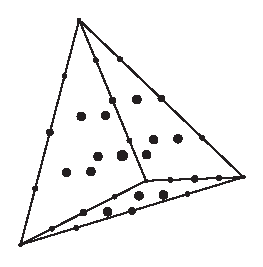
\includegraphics{figures/eps/tetra_popn.eps}}\hspace{4pt}
\caption{\textbf{Population points} }
\label{tetra_popn}
\end{center}
\end{figure}

The diagram (\ref{tetra_popn}) illustrates population points in tetrahedron for $\ell  =  2,  r  =  4$. Populations are represented by dots, 
where smaller dots have lower dispersion and larger dots have higher dispersion.

The variance of the next generation population (with respect to the expected population) (see \cite{Vose1999}) is 
\begin{equation}
\label{RHSvariance}
\mathcal{E}(\| \tau (\bm{p}) - \mathcal{G}(\bm{p}) \|^2) = (1 - \|\mathcal{G}(\bm{p})\|^2) / r
\end{equation}
It follows from Chebyshev's inequality (see \cite{ChebyshevInequality}) that 
\begin{equation}
\label{Cheby}
P(\| \tau (\bm{p}) - \mathcal{G}(\bm{p}) \| \geq \epsilon) \leq \frac{(1 - \|\mathcal{G}(\bm{p})\|^2)} {r{\epsilon}^2}
\end{equation}
where $P$ denotes probability and $\epsilon$ is arbitrary value.

Let $f(r)$ be a function which grows arbitrarily slowly, such that 
\[
\lim_{r \to \infty} f(r)  =  \infty
\]
and
\[
\lim_{r \to \infty} f(r)/\sqrt{r}  =  0.
\]
If $\epsilon  =  f(r)/\sqrt{r}$, then (\ref{Cheby}) becomes
\begin{equation*}
\lim_{r \to \infty} P(\| \tau (\bm{p}) - \mathcal{G}(\bm{p}) \| \geq \epsilon) \; \leq \; \frac{(1 - \|\mathcal{G}(\bm{p})\|^2)} {{f(r)}^2} \; \leq \; 0
\end{equation*}

Therefore, $\tau(\bm{p})$ converges in probability to $\mathcal{G}(\bm{p})$ as the population size increases, 
and $\tau$ corresponds to $\mathcal{G}$ 
in the infinite population case. Moreover, (\ref{RHSvariance}) suggests that the expected distance between finite and 
infinite population in the next generation decreases as $1/\sqrt{r}$.

In Figure (\ref{tetra_popn}), finite population points can be only at certain points, but infinite population can be anywhere on the surface. 
Theorem 3.1 in 'The Simple Genetic Algorithm: Foundations and Theory' states that \emph{if $\bm{p},\bm{q} \;\in\; \Lambda$ are 
arbitrary population vectors for population size $r$, and $\bm{\xi}$ denotes arbitrary element of $\Lambda$, then 
\begin{eqnarray}
\underset{\bm{p} \neq \bm{q}}{inf} \|\bm{p} - \bm{q}\| &\;=\;& \sqrt{2}/r    \label{theorem3.1_a} \\
\underset{\bm{\xi}}{sup} \underset{\bm{p}}{inf} \|\bm{\xi} - \bm{p}\| &\;=\;& O(1/\sqrt{r})     \label{theorem3.1b}
\end{eqnarray}
where the constant (in the "big oh") is independent of the dimension $n$ of $\Lambda$} (see \cite{Vose1999}).
From \ref{theorem3.1_b}, the distance between an infinite population $\bm{\xi}$ and finite population $p$ is at most $O(1/\sqrt{r})$. 
This suggests that the distance between $\tau (\bm{p})$ and $\mathcal{G}(\bm{p})$ might decrease as $1/\sqrt{r}$.

Let $\eta$ be the random variable $\| \bm{q} - \mathcal{G}(\bm{p}) \|$. Let $\phi$ be the convex function $\phi (x) = x^2$. 
Then, $\mathcal{E}(\| \bm{q} - \mathcal{G}(\bm{p}) \|^2)$ becomes $\mathcal{E}(\phi (\eta))$. 
It follows from Jensen's Inequality (see \cite{JensenInequality}) that 
if $\phi$ is a convex function, then
\[
\phi(\mathcal{E}(\eta))) \leq \mathcal{E}(\phi(\eta)) 
\]
Therefore,
\[
\mathcal{E}(\eta) \leq \sqrt{\mathcal{E}(\eta^2)}
\]
Substituting original variables,
\begin{equation}
\label{Jensen}
\mathcal{E}(\| \bm{q} - \mathcal{G}(\bm{p}) \|) \leq \frac{\sqrt{(1 - \|\mathcal{G}(\bm{p})\|^2)}}{\sqrt{\bm{r}}}
\end{equation}
Equation (\ref{Jensen}) bounds the expected rate of convergence for the single-step haploid case; 
the distance is inversely proportional to square root of population size.

Theorem 3.1 from 'The Simple Genetic Algorithm: Foundation and Theory', 
and Jenson's inequality both suggests that the distance between finite population and infinite population decreases like  
$1\sqrt{r}$. But it is all mathematics; what happens when real GA is run? This research explores that 
through simulations in chapter two.

An instance of RHS is called focused if $\mathcal{G}$ is continuously differentiable, and for every $\bm{p}  \in  \Lambda$
the sequence
\[
\bm{p},  \mathcal{G}(\bm{p}),  {\mathcal{G}}^2(\bm{p}),...
\]
converges. $\mathcal{G}$ is also called focused in this case and the path determined by following at each generation what $\tau$ is expected 
to produce will lead to some steady state $\omega$ such that
\[
\mathcal{G}(\omega) = \lim_{n\to\infty} \mathcal{G}(\bm{p}) = \omega.
\]
Such points $\omega$ are called fixed points (or limits) of $\mathcal{G}$. 
And the sequence $\bm{p},  \mathcal{G}(\bm{p}),  {\mathcal{G}}^2(\bm{p}),...$ is called orbit of $\bm{p}$ under $\mathcal{G}$. 
In case of focused $\mathcal{G}$, under some circumstances (conditions explained in chapter three), 
infinite population oscillates converging alternatingly to fixed points (see \cite{Vose1999}). 
If finite population follows infinite population closely, and if infinite population oscillates under certain conditions, then 
does finite population also show oscillating behavior? We investigate whether finite population also oscillates or not with our experiment 
in chapter three. 

If GA forms ergodic Markov chain visiting every population state infinitely often, then $\mathcal{G}$ is also called ergodic. 
Let $\bm{P}_j$ denote $j$th population state in population state vector $P$. Let $\bm{\pi}^k$ be the probability vector having $j$th component 
equal to the probability that $k$th generation population is $\bm{P}_j$. If $\bm{\pi}^0$ is initial distribution and $Q$ is transition matrix, the steady state distribution $\bm{\pi}$ is given by (see \cite{Nix1992})
\[
\lim_{k \to \infty} \bm{\pi}^k \;=\; \bm{\pi}^0 Q^k \;=\; \text{solution to the equation } "\bm{\pi} \; = \; \bm{\pi} Q" 
\]
where $j$th component can be interpreted as relative proporiton of time that GA has a population corresponding tp $\bm{P}_j$. 
If the Markov chain is ergodic, then the steady state is independent of initial population. If GA were to converge to some population $\bm{P}_j$, 
then $\bm{\pi}_j \;=\; 1$ and other components would be $0$. If GA were to oscillate between two populations $\bm{P}_i$ and $\bm{P}_j$, then 
$\bm{\pi}_i \;=\; 1$ and other components $0$ when $k$ = odd generation, and $\bm{\pi}_j \;=\; 1$ and other components $0$ when $k$ = even generation. 
But if GA forms ergodic Markov chain, this does not happen, instead finite population visits every population state infinitely often, and steady state 
distribution $\bm{\pi}$ converges to $\bm{\pi}^\ast$ as population size increases to infinity ( see \cite{Nix1992}) where 
\[
\bm{\pi}^\ast \;=\; \lim_{r \to \infty} \bm{\pi}.
\]
So, in chapter three, we further investigate what happens to finite populations 
if we violate the conditions necessary for population to oscillate, and making GA ergodic.


\section{Overview}
In chapter two, we describe a simple Markov model for diploid case under influence of mutation and crossover. 
The model is non-overlapping, generational, infinite population model assuming random mating and no selective pressure. 
Through abstract development, we show that the diploid model can be specialized by using mask based 
mutation and crossover operators to Vose's infinite population model which is a haploid model. Computational 
simplifications due to reduction of diploid model to haploid model and application of Walsh transform 
are exploited in experimental simulation of model, and through the experiment we demonstrate convergence 
of finite diploid population to infinite population behavior implied by equation \ref{RHSvariance}.

In chapter three, we study evolutionary limits predicted by Vose using infinite population model 
under no selective pressure. We use computation of predicted limits
of infinite population and discuss necessary and sufficient conditions stated by Vose for population
to converge in to periodic orbits. We investigate predicting the convergence of finite population 
short-term behavior to infinite population evolutionary limits under no selective pressure. 
Then it studies case of violation in the necessary and sufficient conditions for population 
to converge periodic orbits. We then study behavior of finite and infinite population when there is 
violation in necessary condition mentioned by Vose.






